\documentclass{article}

\usepackage{fontspec}   %加這個就可以設定字體
\usepackage{xeCJK}       %讓中英文字體分開設置
\setCJKmainfont{標楷體} %設定中文為系統上的字型,而英文不去更動,使用原TeX字型
\setmainfont{Calibri} % 設定英文字型
\XeTeXlinebreaklocale "zh"             %這兩行一定要加,中文才能自動換行
\XeTeXlinebreakskip = 0pt plus 1pt     %這兩行一定要加,中文才能自動換行

\usepackage{titling}
\setlength{\droptitle}{-12em} % 將標題移動至頁面的上面


\title{第四章 - 相機校正/車輪校正/循跡自走車}

\author{陳品維}
\date{} %不要日期

\begin{document}
\maketitle

\section{相機校正}
\subsection{為何需要相機校正}

有幾個因素都需要用到相機校正,像是有時真實世界的座標與相機的座標並不契合,引此需要利用相機校正讓座標互相契合。
\\
\begin{figure}[htp]
    \begin{center}
        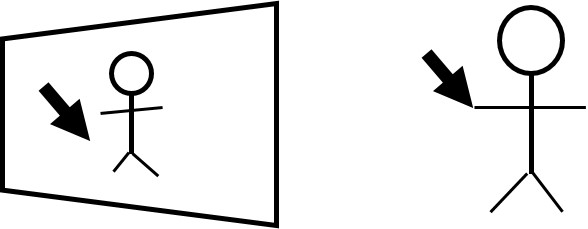
\includegraphics[width=250pt]{pic/圖片1.jpg}
    \end{center}
\end{figure}
\\另外,有時鏡頭本身的誤差或是特性也需要利用相機校正來處理,像是我們所用的鏡頭為廣角的魚眼鏡頭,因此畫面會有扭曲的現象,而藉由相機校正則可以把左邊魚眼扭曲的畫面修正為右邊方正不扭曲的畫面。
\\
\begin{figure}[htp]
    \begin{center}
        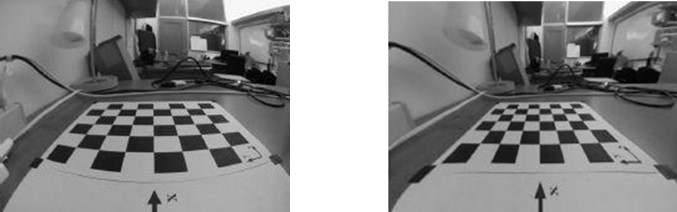
\includegraphics[width=300pt]{pic/圖片2.jpg}
    \end{center}
\end{figure}

\subsection{相機校正運作原理}

相機校正主要分為兩個部分,一個是外部校正,一個是內部校正。外部校正主要是在將世界真實座標與相機座標契合,是一個3D到3D的轉換,至於內部校正,則是把相機的3D影像的座標投影在2D的影像上面。
\\
\begin{figure}[htp]
    \begin{center}
        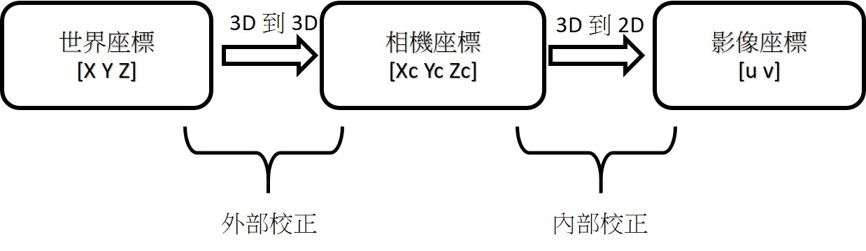
\includegraphics[width=300pt]{pic/圖片3.jpg}
    \end{center}
\end{figure}

我們也可以藉由流程圖更清楚瞭解相機校正的運作。
\\首先內部校正的部分,會先產生有一個內部校正矩陣,它可以幫我們把3D的座標投影到2D的座標,另外內部校正也負責處理失真的問題,包括扭曲及傾斜失真。
\\至於在外部校正的部分,是用來讓真實世界座標與相機座標契合,也就是利用旋轉及移動讓兩個座標契合。
\\
\begin{figure}[htp]
    \begin{center}
        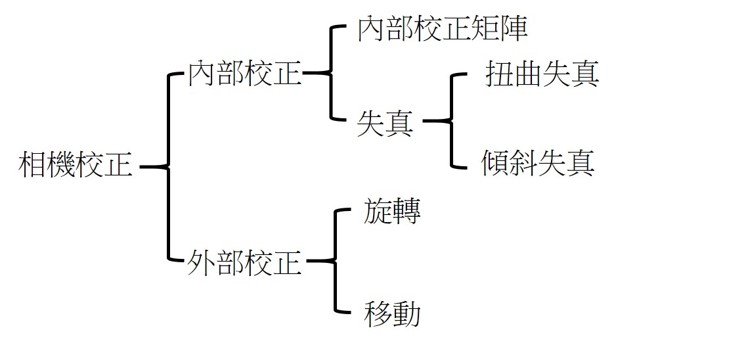
\includegraphics[width=300pt]{pic/圖片4.jpg}
    \end{center}
\end{figure}

下面公式則是相機座標利用數學運算的原理。
\\
\begin{figure}[htp]
    \begin{center}
        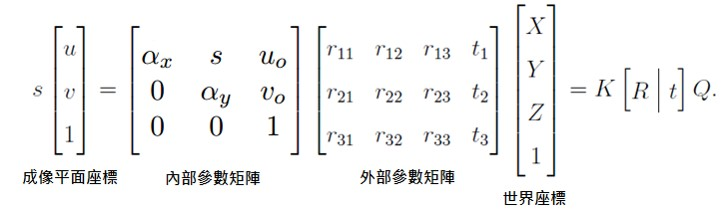
\includegraphics[width=300pt]{pic/圖片5.jpg}
    \end{center}
\end{figure}

\subsection{相機內部校正}

上一節有提過相機內部校正主要分為內部相機矩陣以及處理失真問題,首先我們先來看內部相機矩陣的部分,我們可以看到它就是利用投影的原理將3D座標投影在2D座標上。
\\
\begin{figure}[htp]
    \begin{center}
        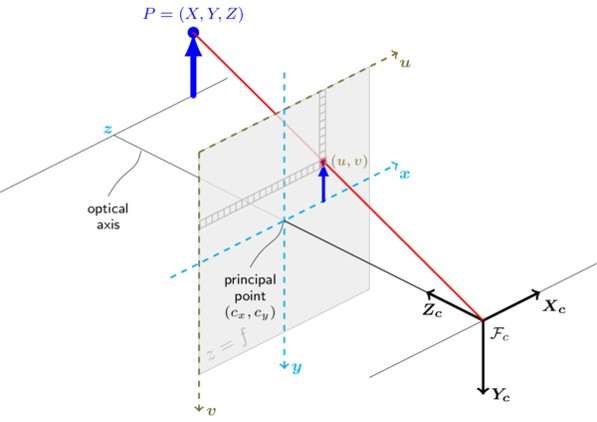
\includegraphics[width=300pt]{pic/圖片6.jpg}
    \end{center}
\end{figure}

內部相機矩陣運算的原理其實很簡單,就是利用相似三角形所得到,影像平面(Image Plane)位在焦距(f)的位置,所以此平面的Z軸座標為f,接這我們利用相似三角形可以得知f/Z=u/X=v/Y,那因為是目的是要轉換到2D平面,所以在Z軸方向可以不需要考慮,因此為了方便計算我們把P點的Z座標設為1,於是可以得到u=fx, v=fy, z=1,最後把它寫成矩陣的形式就可以得到內部相機矩陣。
\\
\begin{figure}[htp]
    \begin{center}
        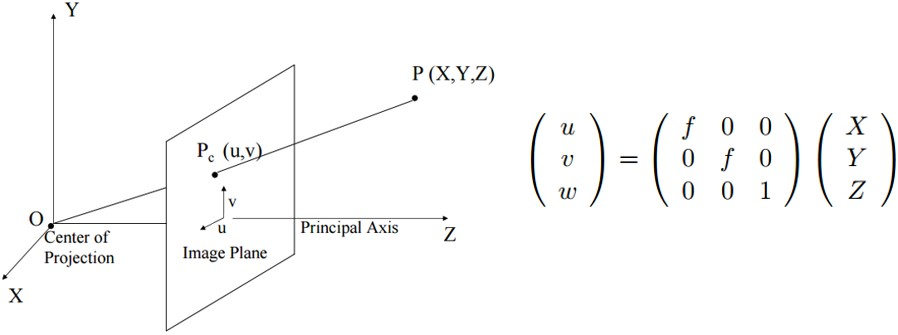
\includegraphics[width=300pt]{pic/圖片7.jpg}
    \end{center}
\end{figure}

但是我們還得考慮一件事,也就是我們剛剛計算的方法是假設影像平面(Image Plane)的中心是剛好位在Z軸上,所以才能理想的使用相似三角形,但大多數的狀況是影像平面的中心不會剛好位在Z軸上,所以我們修正一下上面得到的結果,假如現在影像平面的中心不在Z軸上而在(tu, tv),那我們只要利用平移就可以先把影像中心移到Z軸上,然後再以相似三角形得到內部校正矩陣。
\\
\begin{figure}[htp]
    \begin{center}
        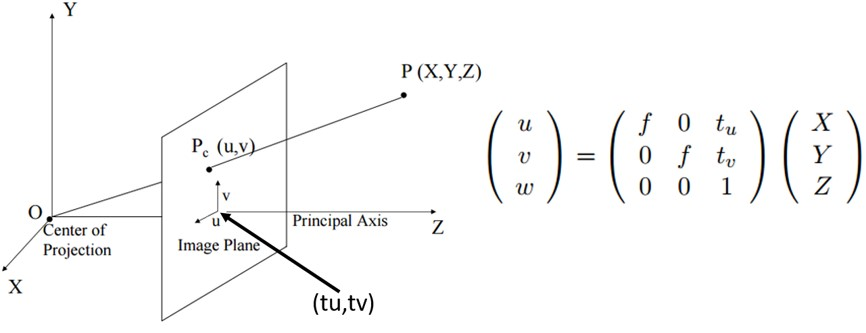
\includegraphics[width=300pt]{pic/圖片8.jpg}
    \end{center}
\end{figure}

在內部校正的部分,我們已經完成內部校正矩陣了,現在我們要處理失真的問題,失真主要分為兩種,一種是扭曲失真,這種問題是因為我們的鏡頭有可能使用魚眼或是其他特殊鏡頭,因此導致扭曲的現象,我們就利用一些校正參數K來修正扭曲的問題。
\\
\begin{figure}[htp]
    \begin{center}
        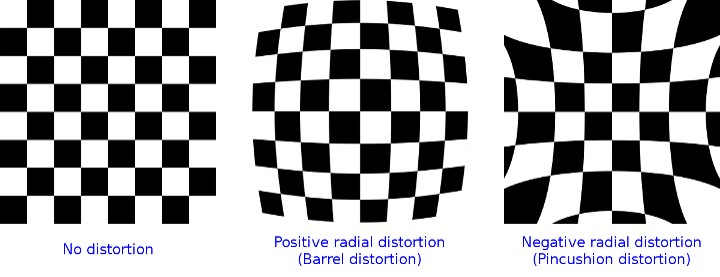
\includegraphics[width=300pt]{pic/圖片9.jpg}
    \end{center}
\end{figure}

另外一種失真是傾斜失真,它發生的原因是因為相機本身的誤差,照道理相機的鏡頭跟感光元件要互相平行,但因為誤差的緣故,會導致感光元件與鏡頭部平行,使得影像失真,我們也可以利用參數p來修正此問題。
\\
\begin{figure}[htp]
    \begin{center}
        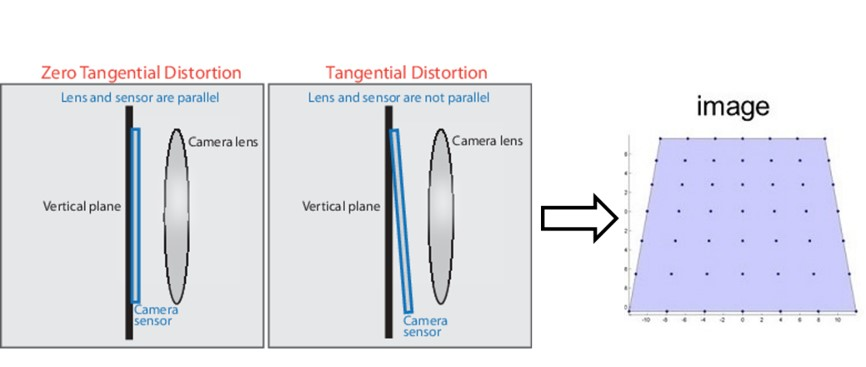
\includegraphics[width=270pt]{pic/圖片10.jpg}
    \end{center}
\end{figure}
\\
利用K及P兩種修正參數,我們可以把影像座標重新校正,運算方法就是利用下面的公式:
\\
\begin{figure}[htp]
    \begin{center}
        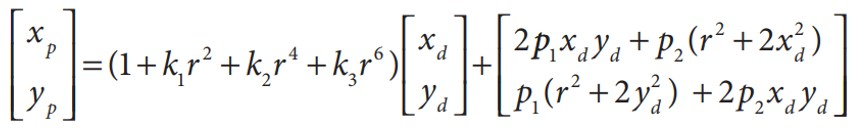
\includegraphics[width=300pt]{pic/圖片11.jpg}
    \end{center}
\end{figure}

在Duckietown中的相機內部校正方法,我們利用棋盤紙及相機捕捉影像並讓openCV計算來達到。我們會讓相機捕捉棋盤紙不同位置的影像,然後利用openCV的intrinsic calibration function不斷去計算相機內部矩陣以及參數k和p,藉此就可以達到相機內部校正了。
\begin{figure}[htp]
    \begin{center}
        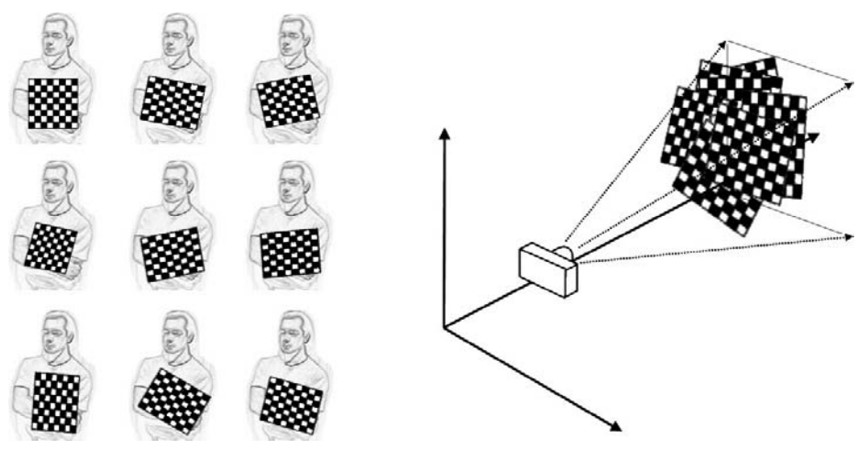
\includegraphics[width=300pt]{pic/圖片12.jpg}
    \end{center}
\end{figure}


\subsection{相機外部校正}

4-1-2已經提過相機外部校正是為了用來把真實世界座標與相機座標契合,這主要分為兩個步驟,一個是旋轉,一個是平移,藉由這兩個步驟,便能把兩個座標互相契合了。
\\
\begin{figure}[htp]
    \begin{center}
        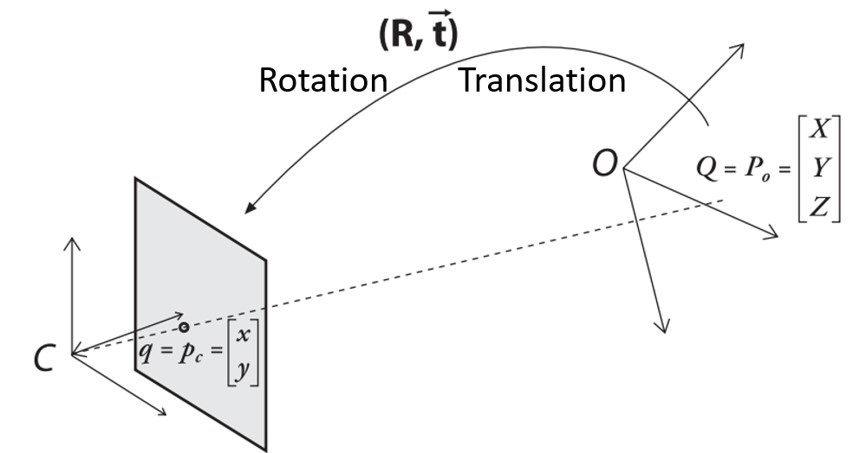
\includegraphics[width=250pt]{pic/圖片13.jpg}
    \end{center}
\end{figure}

在Duckietown中的相機外部校正,我們是先把車子放在一個標記好的定點,然後讓鏡頭照向前方的棋盤紙,而棋盤格的大小以及標記點的位置都是固定好且為已知的,所以我們可以把相機的座標經由旋轉及移動,使得它與已知的真實世界座標契合。
\\
\begin{figure}[htp]
    \begin{center}
        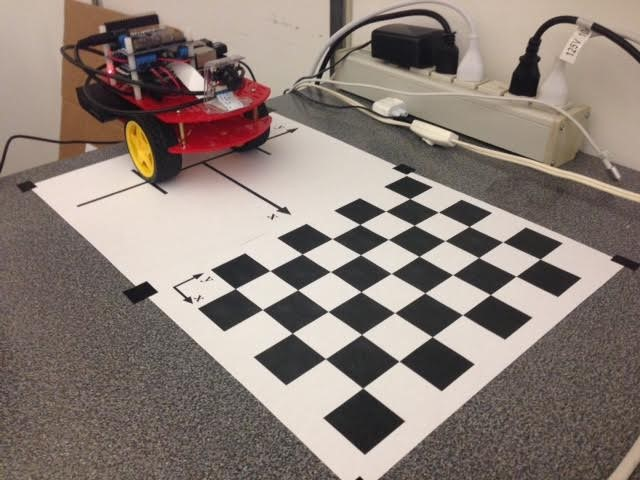
\includegraphics[width=250pt]{pic/圖片14.jpg}
    \end{center}
\end{figure}

\subsection{在Duckiebot上執行相機校正}

接著我們回到我們的車子上,我們要在車子上實現相機校正囉!
\\首先安裝 camera\_calibration node
\\laptop\&duckiebot \$ sudo apt-get install ros-indigo-camera-calibration
\\laptop\&duckiebot \$ sudo vim /etc/ssh/ssh\_config
\\把 “\#ForwardX11 no”  改成 “ForwardX11 yes”  \# 要刪掉

\subsection{Duckiebot相機內部校正}

In laptop, connect laptop and duckiebot to access point
\\duckiebot \$ cd ~/duckietown
\\duckiebot \$ source environment.sh
\\duckiebot \$ source set\_ros\_master.sh duckiebot
\\duckiebot \$ roslaunch duckietown intrinsic\_calibration.launch veh:=duckiebot raw:=true
\\
\\此時會開啟一個視窗,請把棋盤拿至相機前面並以不同位置放置,讓相機蒐集影像樣品。
\\當你蒐集完足夠的影像之後,右上方所有的狀態條將變成綠色,此時 ‘CALIBRATE’ 按鈕就可以點選了。
\\校正將會持續大概10分鐘,如果你很滿意校正完的結果,請按 ‘COMMIT’按鈕,他可以自動將你校正的檔案存進你的車子裡(並不是存在你的電腦裡)
\begin{figure}[htp]
    \begin{center}
        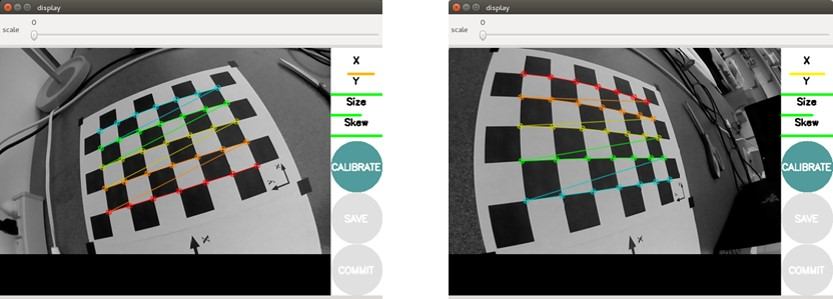
\includegraphics[width=300pt]{pic/圖片15.jpg}
    \end{center}
\end{figure}

\begin{itemize}

\item X bar: 水平移動範圍 (左-右)
\item Y bar: 垂直移動範圍 (上-下)
\item Size bar:棋盤大小範圍 (前-後)
\item Skew bar: 傾斜角範圍

\end{itemize}

校正檔案儲存位置: \~/duckietown/catkin\_ws/src/duckietown/config/baseline/calibration/camera\_intrinsic/veh\_name.yaml
\\
\\確認校正檔案
\\duckiebot\$ cd \~/duckietown/catkin\_ws/src/duckietown/config/baseline/calibration/camera\_intrinsic
\\duckiebot\$ ls
\\你可以看到 “duckiebot.yaml”.
\\duckiebot\$ cat duckiebot.yaml
\\你可以在 duckiebot.yaml裡面看到你的校正參數
\\從Duckietop複製校正檔案到電腦中
\\laptop \$ cd \~/duckietown/catkin\_ws/src/duckietown/config/baseline/calibration/camera\_intrinsic/
\\laptop \$ scp ubuntu@duckiebot.local:\~/duckietown/catkin\_ws/src/duckietown/config/baseline/calibration/camera\_intrinsic/duckiebot.yaml duckiebot.yaml

\subsection{Duckiebot相機外部校正}

把你的車如圖放置:
\\
\begin{figure}[htp]
    \begin{center}
        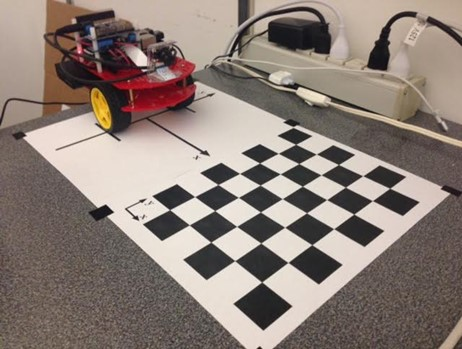
\includegraphics[width=300pt]{pic/圖片16.jpg}
    \end{center}
\end{figure}

開啟 camera \& ground projection
\\duckiebot \$ cd \~/duckietown
\\duckiebot \$ source environment.sh
\\duckiebot \$ source set\_ros\_master.sh duckiebot
\\duckiebot \$ byobu
\\在其中一個終端機上:
\\duckiebot \$ roslaunch duckietown camera.launch veh:=duckiebot raw:=true
\\在另一個終端機上:
\\duckiebot \$ roslaunch ground\_projection ground\_projection.launch  veh:=duckiebot local:=1
\\在電腦中開啟一個終端機
\\laptop \$ cd \~/duckietown
\\laptop \$ source environment.sh
\\laptop \$ source set\_ros\_master.sh duckiebot
\\laptop \$ rostopic list
\\他應該長得像這樣
\\...
\\/$<$VEHICLE\_NAME$>$/camera\_node/camera\_info
\\/$<$VEHICLE\_NAME$>$/camera\_node/image/compressed
\\/$<$VEHICLE\_NAME$>$/camera\_node/image/raw
\\/$<$VEHICLE\_NAME$>$/ground\_projection/lineseglist\_out
\\/$<$VEHICLE\_NAME$>$/line\_detector\_node/segment\_list
\\/rosout
\\/rosout\_agg
\\...
\\laptop \$ rosservice list
\\...
\\/veh\_name/ground\_projection/estimate\_homography
\\/veh\_name/ground\_projection/get\_ground\_coordinate
\\...
\\估測 homography
\\laptop \$ rosservice call /duckietbot/ground\_projection/estimate\_homography
\\homography檔案會在下列位置處找到
\\\~/duckietown/catkin\_ws/src/duckietown/config/baseline/calibration/camera\_extrinsic/duckiebot.yaml
\\從Duckietop複製校正檔案到電腦中
\\laptop \$ cd \~/duckietown/catkin\_ws/src/duckietown/config/baseline/calibration/camera\_extrinsic/
\\laptop \$ scp ubuntu\@duckiebot.local:\~/duckietown/catkin\_ws/src/duckietown/config/baseline/calibration/camera\_extrinsic/duckiebot.yaml duckiebot.yaml

\subsection{上傳校正檔案到Github repo}

觀察你所改變的檔案
\\laptop \$ cd \~/duckietown
\\laptop \$ git status
\begin{figure}[htp]
    \begin{center}
        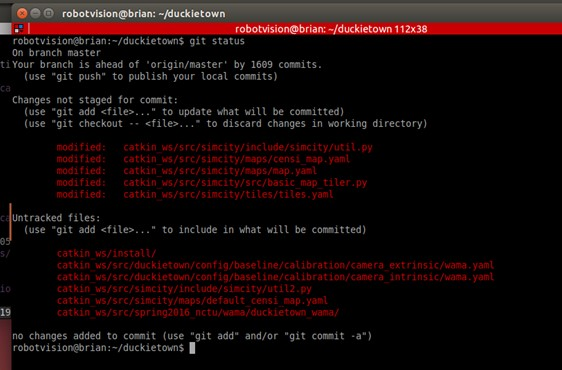
\includegraphics[width=300pt]{pic/圖片17.jpg}
    \end{center}
\end{figure}

你所更改的檔案將會變成紅色
\\Git add \& commit \& push
\\laptop \$git add catkin\_ws/src/duckietown/config/baseline/calibration/camera\_extrinsic/ duckiebot.yaml catkin\_ws/src/duckietown/config/baseline/calibration/ camera\_intrinsic/duckiebot.yaml
\\Add 兩個校正檔
\\laptop \$ git status
\\
\begin{figure}[htp]
    \begin{center}
        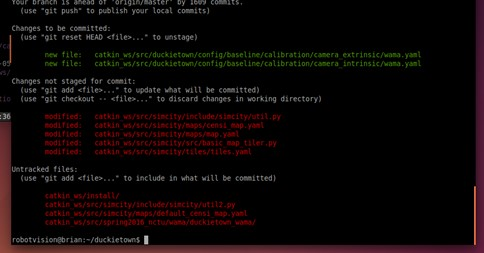
\includegraphics[width=300pt]{pic/圖片18.jpg}
    \end{center}
\end{figure}

當add完以後檔案將會呈現綠色
\\laptop \$ git commit -m "duckiebot camera calibration"
\\laptop \$ git push

\subsection{測試內部校正結果}

比較 /image\_mono 和 /image\_rec
\\比較扭曲的棋盤和沒有扭曲的棋盤
\\如同外部校正時所擺放的樣子:

\begin{figure}[htp]
    \begin{center}
        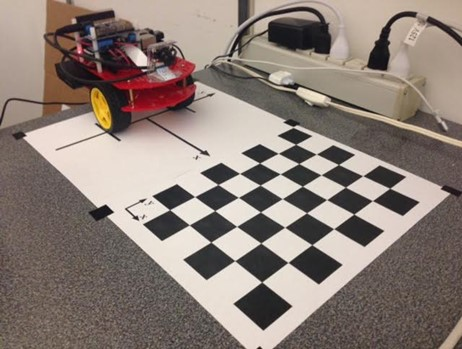
\includegraphics[width=300pt]{pic/圖片19.jpg}
    \end{center}
\end{figure}

duckiebot \$ cd \~/duckietown
\\duckiebot \$ source environment.sh
\\duckiebot \$ source set\_ros\_master.sh duckiebot
\\duckiebot \$ byobu
\\在其中一個終端機上:
\\duckiebot \$ roslaunch duckietown camera.launch veh:=duckiebot raw:=true
\\在另一個終端機上:
\\duckiebot \$ roslaunch duckietown\_unit\_test ground\_projection\_test1.launch veh:=duckiebot  rectify:=true
\\duckiebot \$ sudo apt-get install ros-indigo-image-view ros-indigo-rosbash
\\
\\image\_mono
\\duckiebot \$ rosrun image\_view image\_view image:=/duckiebot/camera\_node/image\_mono
\\當你按右鍵,他會把影像存成 frame0000.jpg
\\image\_rec
\\duckiebot \$ rosrun image\_view image\_view image:=/duckiebot/camera\_node/image\_rect
\\當你按右鍵,他會把影像存成 frame0000.jpg
\begin{figure}[htp]
    \begin{center}
        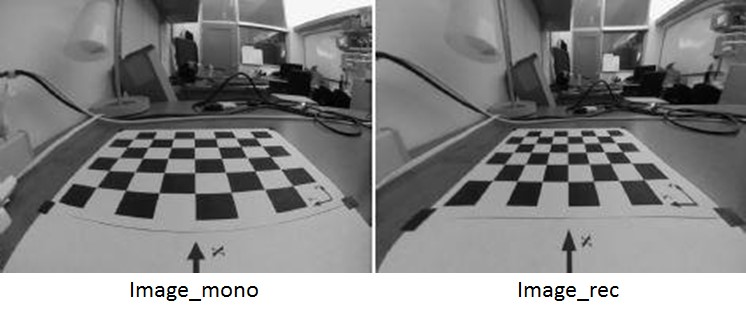
\includegraphics[width=300pt]{pic/圖片20.jpg}
    \end{center}
\end{figure}

\subsection{測試外部校正結果}

測試 ground projection
\\In laptop, connect laptop and duckiebot to access point
\\duckiebot \$ cd \~/duckietown
\\duckiebot \$ source environment.sh
\\duckiebot \$ source set\_ros\_master.sh duckiebot
\\duckiebot \$ byobu
\\在其中一個終端機上:
\\duckiebot \$ roslaunch duckietown camera.launch veh:=duckiebot raw:=true
\\在另一個終端機上:
\\duckiebot \$ roslaunch duckietown\_unit\_test ground\_projection\_test1.launch veh:=duckiebot  rectify:=true
\\和ground truth coordinates做比較
\\
\\duckiebot \$ rosrun ground\_projection test\_projection.py duckiebot
\\
\\他會顯示當前的影像,當你點及影像中的圖片時,他會回傳那個點的ground座標
\\
\begin{figure}[htp]
    \begin{center}
        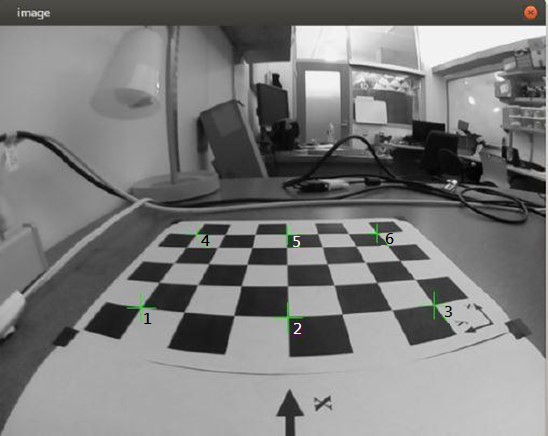
\includegraphics[width=300pt]{pic/圖片21.jpg}
    \end{center}
\end{figure}

按照上方順序點取所標示的六個點,他會回傳如下資訊:
\\
\\image coordinate: (168, 331)
\\normalized image coordinate: (0.262500, 0.689583)
\\ground coordinate: (0.192808, 0.094423, 0.000000)
\\image coordinate: (341, 341)
\\normalized image coordinate: (0.532813, 0.710417)
\\ground coordinate: (0.190528, 0.002201,0.000000)
\\image coordinate: (511, 328)
\\normalized image coordinate: (0.798438, 0.683333)
\\ground coordinate: (0.191026, 0.095562,0.000000)
\\image coordinate: (234, 245)
\\normalized image coordinate: (0.365625, 0.510417)
\\ground coordinate: (0.304039, 0.085974, 0.000000)
\\image coordinate: (339, 245)
\\normalized image coordinate: (0.529687, 0.510417)
\\ground coordinate: (0.300432, 0.003149,0.000000)
\\image coordinate: (445, 244)
\\normalized image coordinate: (0.695312, 0.508333)
\\ground coordinate: (0.297958, 0.090594,0.000000)
\\此六個點的 ground truth 座標為:
\\1.(0.191, 0.093, 0.0)
\\2.(0.191, 0.0, 0.0)
\\3.(0.191, 0.093,0.0)
\\4.(0.315, 0.093, 0.0)
\\5.(0.315, 0.0, 0.0)
\\6.(0.315, 0.093,0.0)
\\與ground truth做比較,注意比較近的點(1, 2, 3) 會有比較小的誤差 (大約 1~2 millimeter), 然而比較遠的點 (4, 5, 6) 有相對比較大的誤差 (大約 1~2 centimeter)。
\\
\\如果你的ground coordinates和ground truth coordinates相似的話,你的相機校正就告一個段落,按 ‘ESC’ 離開

\section{車輪校正}

\subsection{為何需要車輪校正?}

車輪校正的主要目的有兩個,首先,是為了要修正機硬體上所產生的誤差,像是車子明明要走直線,卻偏向了右邊,第二個目的,是要調整車子的速度,以免在循跡駕駛時,車速過快導致偏移軌道。
\\
\begin{figure}[htp]
    \begin{center}
        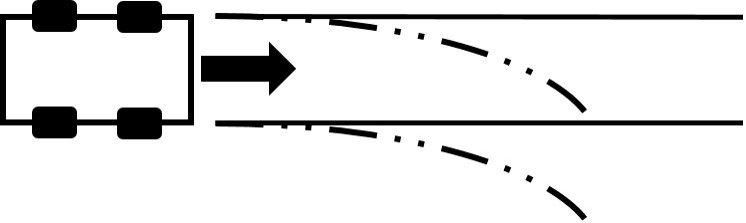
\includegraphics[width=300pt]{pic/圖片22.jpg}
    \end{center}
\end{figure}
車子會無法走直線的原因有很多種,主要是硬體方面的誤差所導致,像是兩邊的輪子大小可能會不太相同,抑或是車上所放置的行動電源等物體導致車子左右重量不均,都有可能導致車子無法走直線,因此我們利用改變兩邊馬達的PWM輸出,使得車子能夠走直線。至於在快慢的部分,則是改變gain,也就是改變馬達的電壓輸出讓車子能達到自己想要的速度。
\\
\begin{figure}[htp]
    \begin{center}
        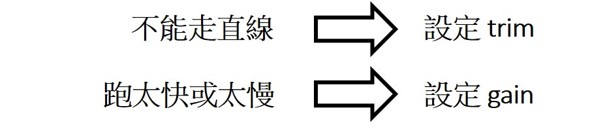
\includegraphics[width=300pt]{pic/圖片23.jpg}
    \end{center}
\end{figure}

\subsection{在Duckiebot上執行輪子校正}

duckiebot $ cd ~/duckietown
\\duckiebot $ source environment.sh
\\duckiebot $ source set_ros_master.sh duckiebot
\\duckiebot $ byobu
\\
\\確定你的車有連接到wifi
\\開啟joystick
\\在byobu中其中一個終端機:
\\duckiebot: \$ roslaunch duckietown\_demos joystick.launch veh:=duckiebot
\\
\\調整參數
\\改到 0.01:
\\在byobu中另一個終端機:
\\duckiebot: \$ rosservice call /duckiebot/inverse\_kinematics\_node/set\_trim -- 0.01 
\\duckiebot: \$  rosservice call /duckiebot/inverse\_kinematics\_node/set\_trim 0.01 
\\
\\或是往負的方向調整, 例如: -0.01:
\\duckiebot: \$ rosservice call /duckiebot/inverse\_kinematics\_node/set\_trim -- -0.01 
\\
\\持續調整直到車子可以走直線
\\
\\設定gain
\\duckiebot: \$ rosservice call /duckiebot/inverse\_kinematics\_node/set\_gain -- 1.1 
\\
\\儲存參數
\\duckiebot: \$ rosservice call /duckiebot/inverse\_kinematics\_node/save\_calibration 
\\
\\如果你是第一次做,他會創造一個 duckiebot.yaml 檔,並儲存在下列資料夾 :
\\\~/duckietown/catkin\_ws/src/duckietown/config/baseline/calibration/kinematics
\\
\\把校正檔案從車子複製到電腦中
\\laptop \$ cd \~/duckietown/catkin\_ws/src/duckietown/config/baseline/calibration/kinematics
\\laptop \$ scp ubuntu@duckiebot.local:\~/duckietown/catkin\_ws/src/duckietown/config/baseline/calibration/kinematics/duckiebot.yaml duckiebot.yaml

\section{有限狀態機Finite State Machine(FSM)}

\subsection{為何需要有限狀態機?}

首先設著想一下下圖的情況,如果現在有一台車子放在軌道上,照道理它會循跡自走,所以他應該要右轉,但是這時我們又用遙控器叫它向左轉,踏它到底該選擇循跡自走向右轉還是選擇聽從遙控器的指令向右呢?於是這時候我們就需要有限狀態機來幫我們,有限狀態機主要由”事件”和”狀態”組成,也就是當我們遇到一個特定的事件,它就會跳到特定的狀態,藉此車子就會知道他這時到底該循跡還是該聽從遙控器。
\begin{figure}[htp]
    \begin{center}
        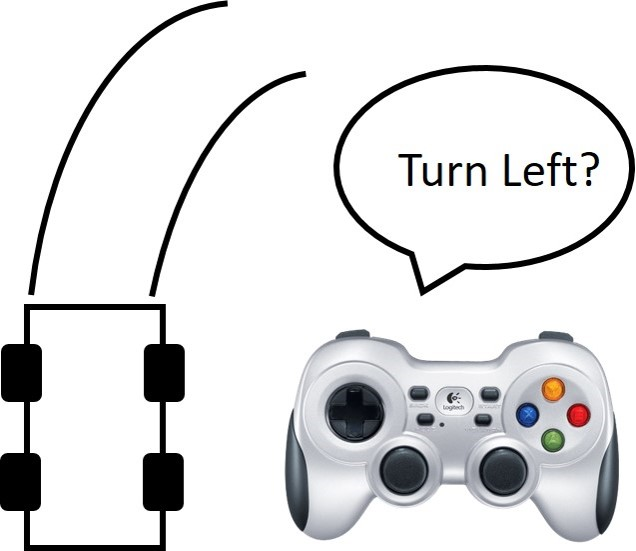
\includegraphics[width=200pt]{pic/圖片24.jpg}
    \end{center}
\end{figure}
\\
以duckietown為例,我們只要”按下LB鍵”這個事件發生,車子就會跳到”循跡自走”這個狀態,而當我們有”按下start鍵”這個事件發生,車子就會跳到”搖控器控制”這個狀態,因此藉由有限狀態機,車子就不會感到困惑說到底該向左還是向右,因為它會遵循事件而跳到特定的狀態。

\begin{figure}[htp]
    \begin{center}
        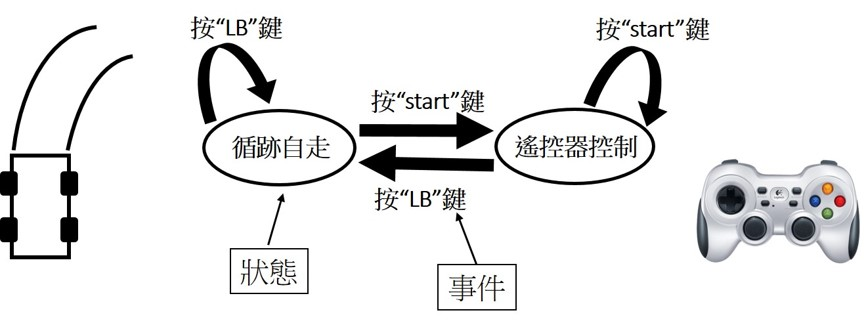
\includegraphics[width=300pt]{pic/圖片25.jpg}
    \end{center}
\end{figure}

\subsection{Duckietown中的有限狀態機}

下圖是Duckietown完整的有限狀態機示意圖

\begin{figure}[htp]
    \begin{center}
        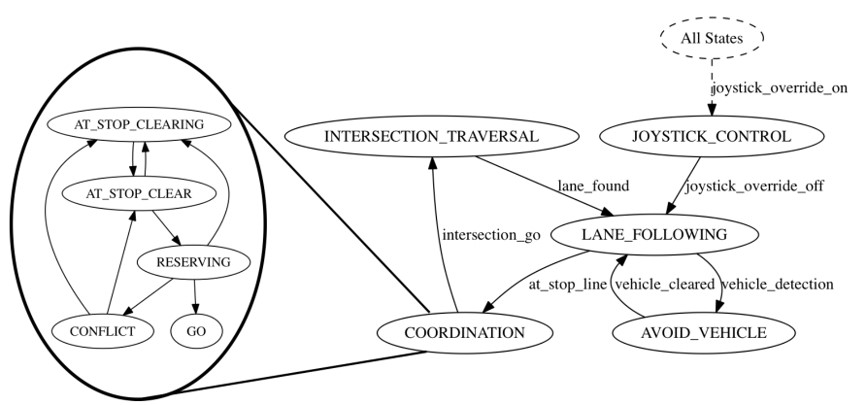
\includegraphics[width=300pt]{pic/圖片26.jpg}
    \end{center}
\end{figure}

有限狀態機是在\~/duckietown/catkin\_ws/src/duckietown/config/baseline/fsm/fsm\_node/default.yaml這個檔案中所設定的,以下圖部分程式碼為例,我們可以看到現在車子是搖控器控制(JOYSTICK CONTROL)的狀態,所以當我們遇到”joystick\_override\_off”這個事件時,車子就會跳到循跡自走(LANE\_FOLLOWING)的狀態,那下方active\_node是在說在搖控器控制(JOYSTICK CONTROL)這個狀態下所要開啟的node。
\\

\begin{figure}[htp]
    \begin{center}
        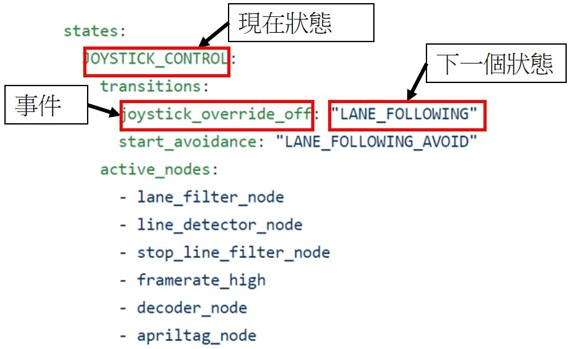
\includegraphics[width=300pt]{pic/圖片27.jpg}
    \end{center}
\end{figure}

\subsection{車子命令控制}

回到剛剛的情境,假如現在我們已經利用有限狀態機讓車子知道該到哪個狀態了,例如說現在我們按下了”start”鍵讓車子進入搖控器控制的狀態,但是我們是怎麼讓車子一進到這個狀態,便只聽從遙控器的指令而不是軌跡所給的指令呢?這就是靠著車子命令控制的幫忙來達成。
\begin{figure}[htp]
    \begin{center}
        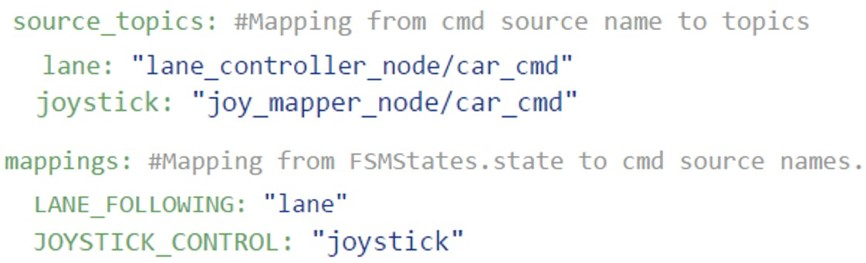
\includegraphics[width=300pt]{pic/圖片28.jpg}
    \end{center}
\end{figure}
我們可以看到\~/duckietown/catkin\_ws/src/duckietown/config/baseline/dagu\_car/car\_cmd\_switch\_node/default.yaml這個檔案,下圖是部分程式碼的截圖。
\\
\\我們可以先看到mappings的部分,它列了很多狀態及相對應的關鍵字,像是LANE\_FOLLOWING這個狀態就對應到lane這個關鍵字,JOYSTICK\_CONTROL這個狀態就對應到joystick這個關鍵字。
\\
\\接著我們再看到source\_topics的部分,我們換看到他列出很多關鍵字對應到特定的topic,例如lane這個關鍵字對應到tane\_controller\_node/car\_cmd這個topic,joystick這個關鍵字對應到joy\_mapper\_node/car\_cmd這個關鍵字。
\\
\\所以這時候我們就明瞭了,當現在的狀態是在循跡自走(LANE\_FOLLOWING)時,它就會經由關鍵字對應到lane\_controller\_node/car\_cmd這個topic,所以在這個狀態,它只會聽從這個topic的指令,藉此達到車子命令控制。
\\

\subsection{循跡自走車}

在處理完相機校正以及輪胎校正後,現在你的車子已經可以完成循跡自走囉,所以現在我們試著去執行lane following了。
\\下載所需軟件:
\\duckiebot \$ sudo apt-get install libblas-dev liblapack-dev libatlas-base-dev gfortran -y
\\
\\執行 lane following:
\\duckiebot \$ cd \~/duckietown
\\duckiebot \$ source environment.sh
\\duckiebot \$ source set\_ros\_master.sh duckiebot
\\duckiebot \$ source set\_vehicle\_name.sh duckiebot
\\duckiebot \$ roslaunch duckietown\_demos lane\_following.launch veh:=duckiebot line\_detector\_param\_file\_name:=universal
\\
\\設定FSM:
\\laptop \$ cd \~/duckietown
\\laptop \$ source environment.sh
\\laptop \$ source set\_ros\_master.sh duckiebot
\\laptop \$ rosservice call /duckiebot/fsm\_node/set\_state LANE\_FOLLOWING


\end{document}